% -----------------------------------------------------------------------------
%   Arquivo: ./01-texto/desenvolvimento.tex
% -----------------------------------------------------------------------------


\section{Desenvolvimento}\label{sec:desenvolvimento}

Antes de se desenvolver o código da solução para o problema proposto, é preciso entender os desafios que acompanham este problema. São eles: 
\noindent\textbf{(1)} Encontrar um volume de dados suficiente para o aprendizado 
\noindent\textbf{(2)} Como transformar e modelar esses dados de forma a se transformar numa entrada plausível para o modelo matemático? 
\noindent\textbf{(3)} Qual o melhor algoritmo de aprendizado para a predição?

\subsection{Primeiro desafio}

Para o primeiro desafio, é preciso frisar que todos os tipos de problemas que são resolvidos com aprendizado de máquina supervisionado devem ter um conjunto de dados de treinamento de tamanho satisfatório com o objetivo de cobrir todas as possibilidades e saídas, assim permitindo que o algoritmo 'conheça' todo o escopo do problema e possa gerar saídas com grande nível de precisão.

No tocante à predição de resultados de partidas de futebol isso não é diferente. É necessário uma grande base de dados que contenha o histórico de milhares de partidas de futebol de  várias temporadas. Por isso, foram estudados diversos conjuntos de dados e foi selecionado o conjunto de dados chamado 'European Soccer Database', que contém uma amostra de 25 mil partidas da principal liga de onze países da Europa entre os anos de 2008 e 2016.

Mais detalhadamente falando, essa base de dados possui informações sobre jogos de futebol, jogadores, equipes, países, campeonatos e habilidades técnicas de jogadores. Trata-se de um conjunto de dados bastante completo e apto a ser usado para a modelagem do problema proposto.

\subsection{Segundo desafio}

Com a base de dados em mãos, foi necessário um estudo sobre como preparar os dados de entrada das amostras para servirem de dados de entrada para o algoritmo de aprendizado. A primeira decisão tomada foi a de não usar 100\% dessas amostras, uma vez que em cada um dos onze países contidos na base de dados as influências no resultado de um jogo e até mesmo a maneira de praticar o esporte é diferente. Ou seja, há variáveis que influenciam mais do que outras no resultado de uma partida em um determinado campeonato, e essas variáveis podem influenciar menos em detrimento de outras em outra liga de outro país.


% -----------------------------------------------------------------------------
% Nova subseção
% -----------------------------------------------------------------------------

\subsection{Figura ocupando uma coluna}		% edite para alterar o título da subseção

A \textbf{Figura \ref{fig:patoA}} foi inserida, em uma única coluna, utilizando os comandos abaixo.

\begin{center}
  \captionof{figure}{Pato na lagoa. Fator de escala: 8\% da original} 
  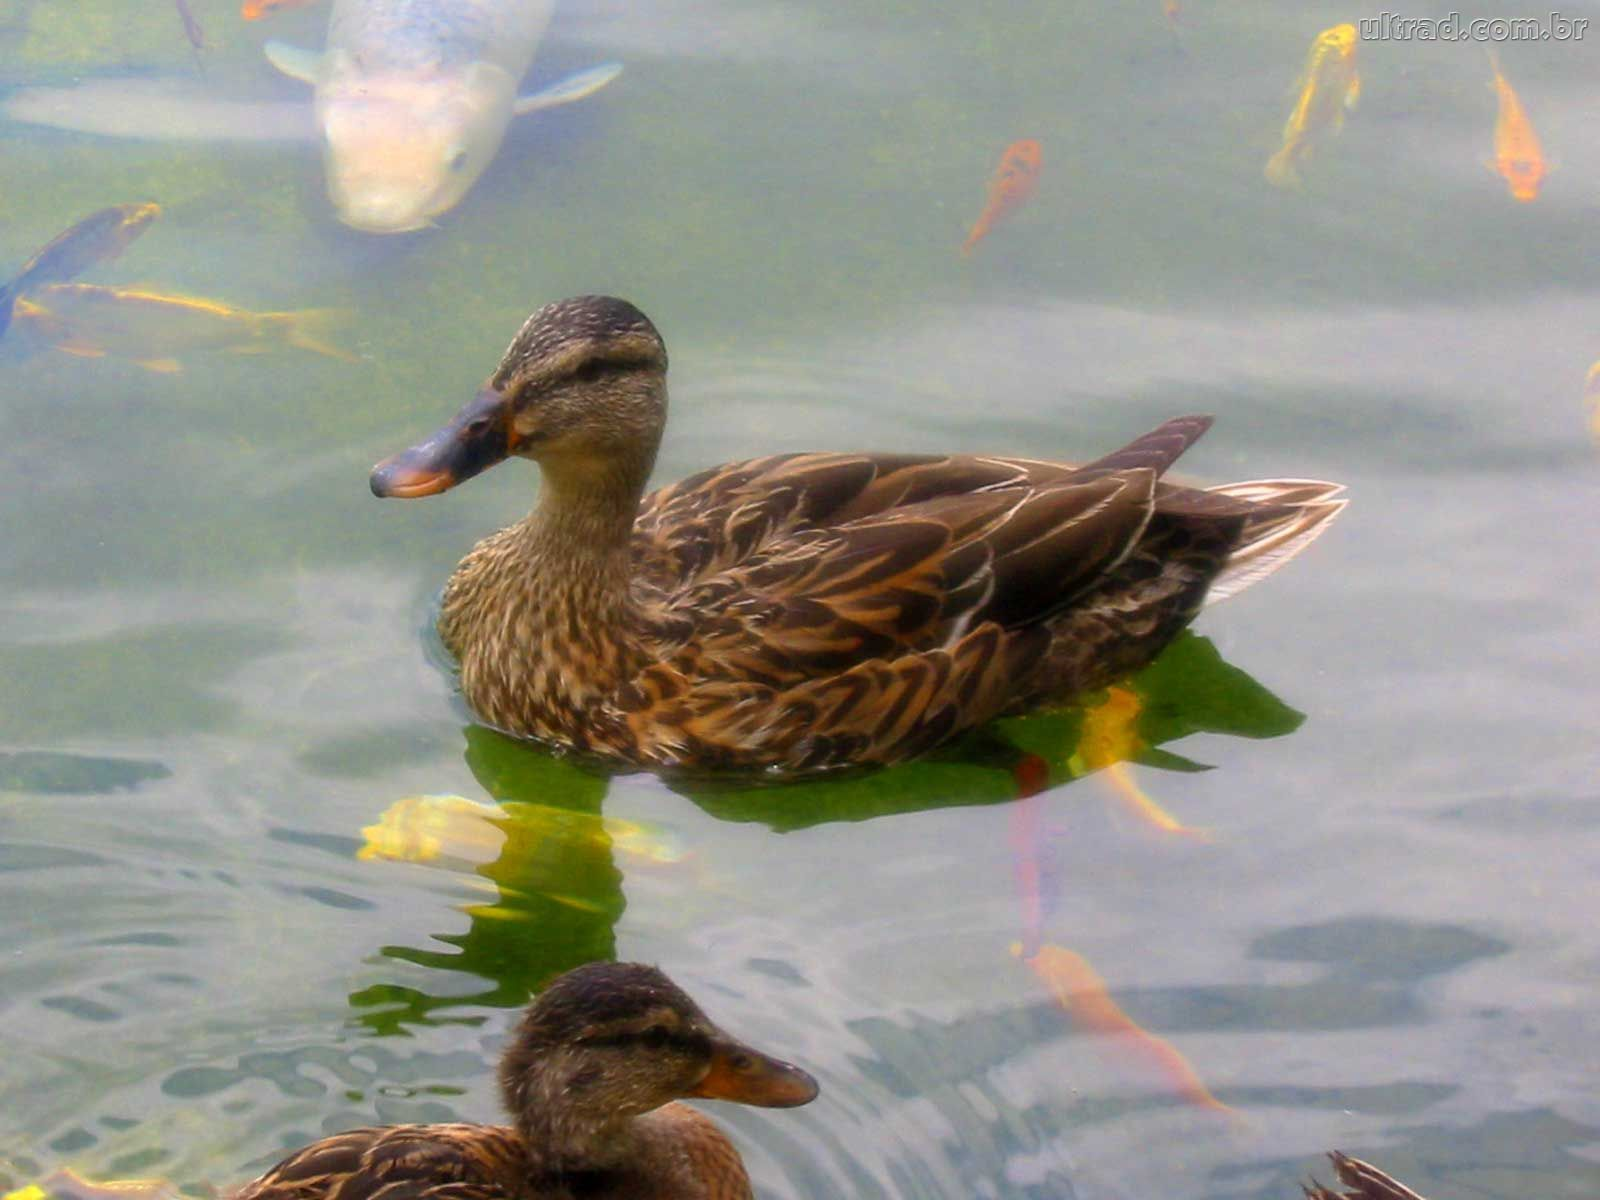
\includegraphics[scale=0.08]{./02-figuras/pato}
  \label{fig:patoA}
\end{center}

Artigos como mais de duas colunas não suportam o ambiente "figure" utilizado neste modelo \LaTeX. Uma alternativa para este problema é a inclusão do pacote:

{\tiny
\begin{verbatim}
    \usepackage{caption}
\end{verbatim}
}

e das seguintes linhas de comando:

{\tiny
\begin{verbatim}
    \begin{center}
      \captionof{figure}{<caption da figura>} 
      \includegraphics[<comandos alternativos>]
      		{<caminho ou nome da figura>}
      \label{<nome da referencia da figura>}
    \end{center}
\end{verbatim}
}



% -----------------------------------------------------------------------------
% Nova subseção
% -----------------------------------------------------------------------------

\subsection{Figura ocupando duas colunas} 		% edite para alterar o título da subseção

O ambiente \verb+figure+ pode ser usado em um artigo quando a figura for centralizada entre as margens do artigo (ocupa um espaço maior que uma coluna). Porém é necessário a introdução do \verb+*+ após o comando \verb+figure+.

\begin{figure*}
	\centering
	\caption{Pato na lagoa. Fator de escala: 20\% da original} 
	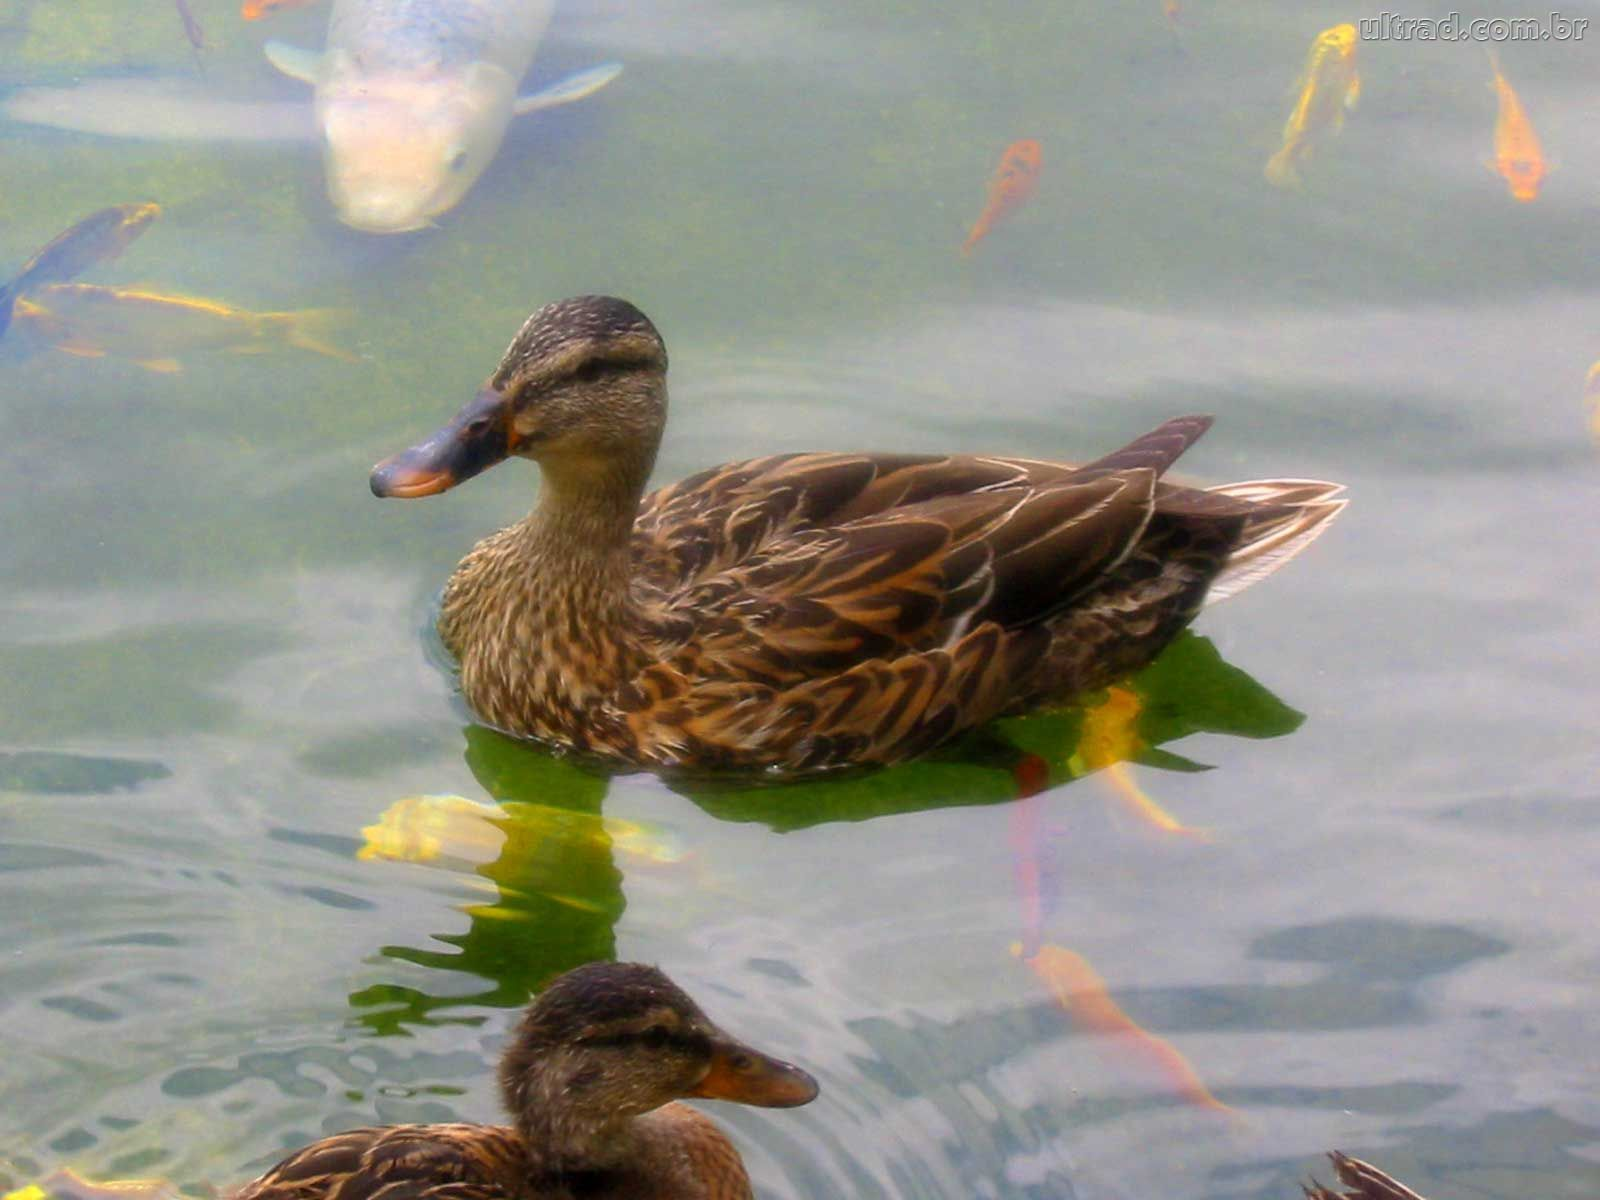
\includegraphics[scale=0.2]{./02-figuras/pato}
	\label{fig:patoB}
\end{figure*}

A \textbf{Figura \ref{fig:patoB}} foi inserida no artigo utilizando o comando \verb+figure*+ para o ambiente de figura.

{\tiny
\begin{verbatim}
   \begin{figure*}
     \centering
     \caption{Pato na lagoa. Fator de escala: 20\% da original} 
     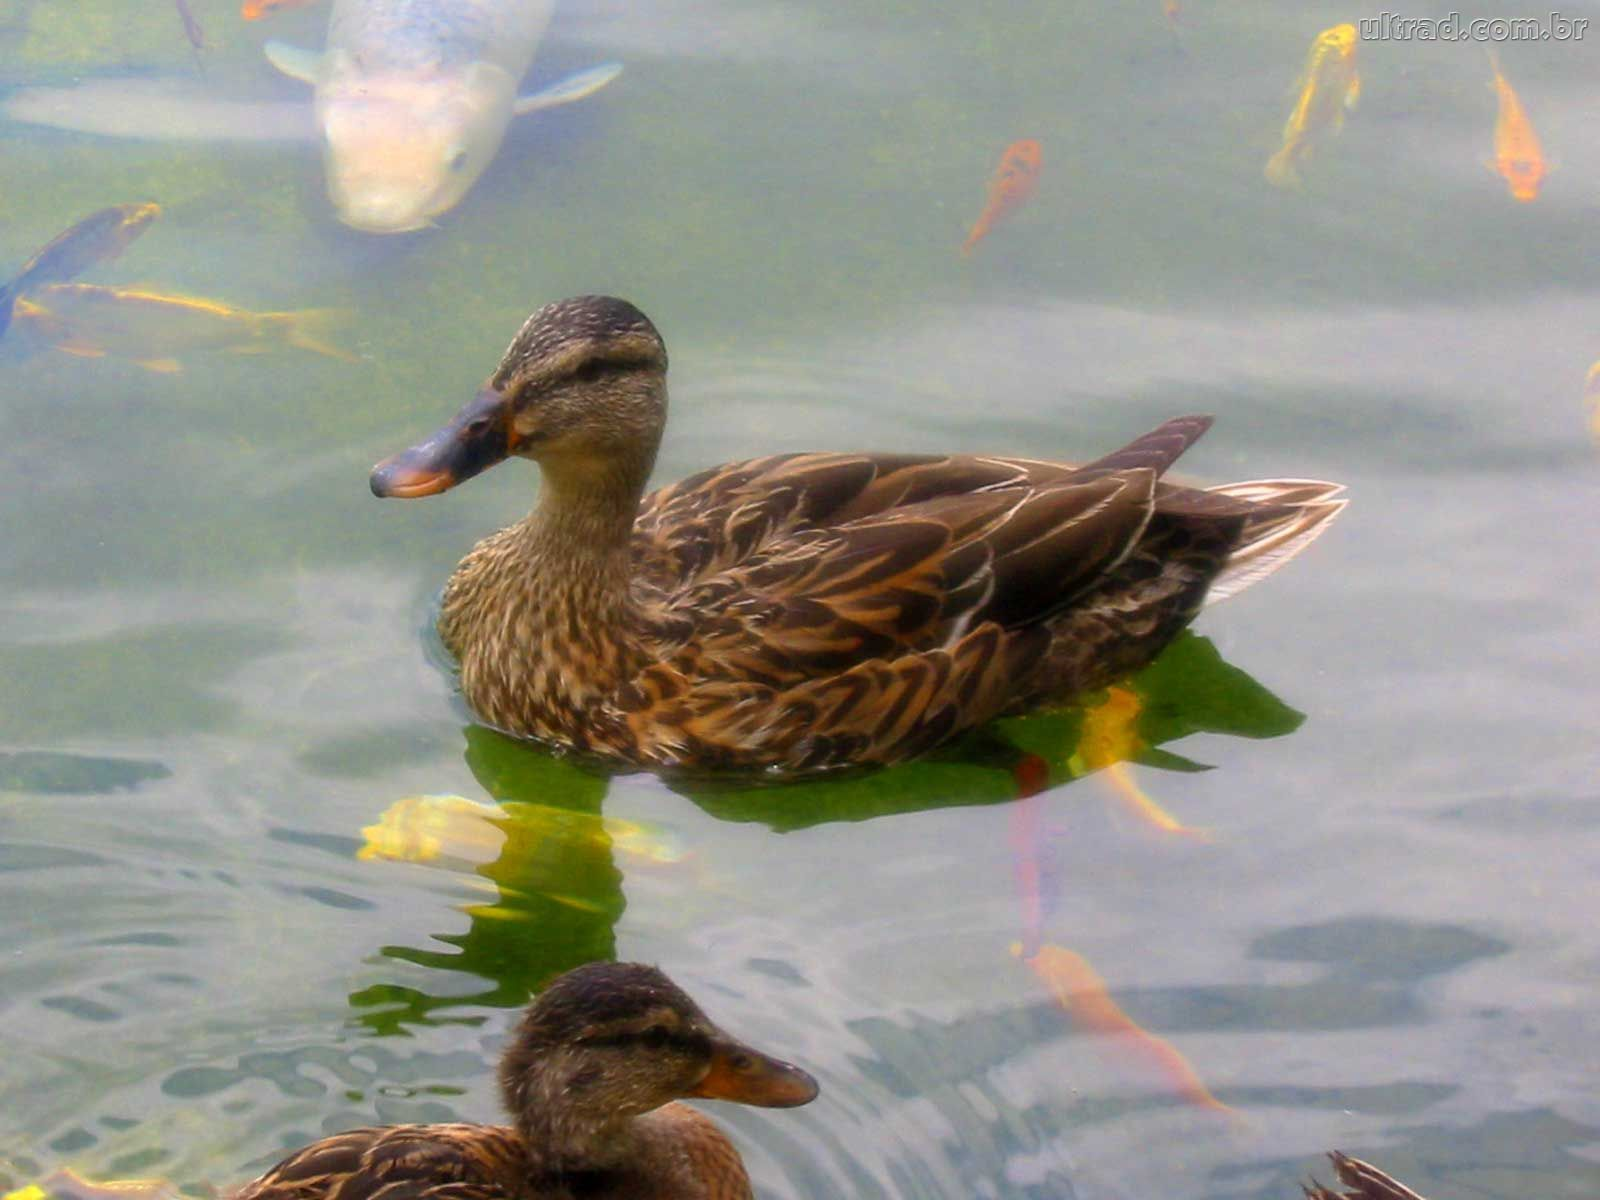
\includegraphics[scale=0.2]{./02-figuras/pato}
     \label{fig:patoB}
   \end{figure*}
\end{verbatim}
}



% -----------------------------------------------------------------------------
% Nova subseção
% -----------------------------------------------------------------------------

\subsection{Tabelas} 		% edite para alterar o título da subseção

O ambiente de tabelas é inserido no texto de modo análogo àquele feito no ambiente de figuras.




% -----------------------------------------------------------------------------
% Nova subseção
% -----------------------------------------------------------------------------

\subsection{Citações de referências} 		% edite para alterar o título da subseção

As referências são inseridas no texto como em qualquer documento em \LaTeX. Quando o nome do autor da referência faz parte do texto que você está escrevendo use o comando  \verb+\citeonline{}+ e quando este não for o caso use o comando \verb+\cite{}+. Veja a diferença entre os dois nas seguintes frases:

\noindent\textbf{(1)} Conforme discute \citeonline{kim1996} o resultado [...].

\noindent\textbf{(2)} Alternativamente a literatura\cite{kim1996} indica que o resultado [...].

Quando se tem mais de uma referência a ser citada em um mesmo certo trecho, há duas possibilidades de referenciá-las:

\noindent\textbf{(1)} colocar todas as referências em um único colchete (\emph{i.e.}, num mesmo comando \verb+\cite+),


\cite{kim1996,Wikibooks2009}

	
\noindent\textbf{(2)} colocar cada referência em seu próprio colchete (\emph{i.e.}, usando vários comandos \verb+\cite+ consecutivos),


\cite{kim1996}\cite{Wikibooks2009}

